\section{Experimental Results}
\label{sec:experimental_results}

This section presents the results of our empirical evaluation, addressing the four research questions defined in Section~\ref{sec:introduction}. We analyze the impact of multi-agent orchestration, model specialization, adaptive routing, and prompt repetition on code generation performance. Additionally, we provide an in-depth analysis of escalation patterns, tier distribution, and static code quality metrics.

All results are based on the execution of 164 tasks from the HumanEval benchmark. 
% -----------------------------------------------------------------------------
\subsection{RQ1: Effect of Multi-Agent Architecture}
\label{subsec:rq1_results}

We first investigate whether a multi-agent pipeline with role separation improves functional correctness compared to a single-agent baseline. We compare \textbf{Architecture A} (Single-Agent) and \textbf{Architecture B} (Multi-Agent), both using the Qwen2.5-Coder-7B-Instruct model for all roles.

Table~\ref{tab:rq1_results} summarizes the performance metrics. Architecture B achieved a pass rate of \textbf{72.6\%}, representing a significant improvement of 4.9 percentage points over the single-agent baseline (67.7\%). The non-overlapping confidence intervals suggest this difference is statistically meaningful.

\begin{table}[ht]
    \centering
    \caption{Comparison of Single-Agent (A) vs Multi-Agent (B) Architectures.}
    \label{tab:rq1_results}
    \resizebox{\columnwidth}{!}{
    \begin{tabular}{lcccc}
        \toprule
        \textbf{Architecture} & \textbf{Pass Rate} & \textbf{Pass@1} & \textbf{95\% CI} & \textbf{Passed/Total} \\
        \midrule
        A (Single-Agent) & 67.7\% & 67.7\% & [60.2, 74.4] & 111/164 \\
        B (Multi-Agent)  & \textbf{72.6\%} & 50.6\% & [65.3, 78.8] & 119/164 \\
        \bottomrule
    \end{tabular}
    }
\end{table}

The Pass@1 metric for Architecture B (50.6\%) refers to the success rate of the first Developer attempt before any Reviewer feedback or retry loops. Notably, this is lower than Architecture A's single-shot performance (67.7\%), that obiously has no retry loops. However, the multi-agent retry mechanism (where the Reviewer analyzes test failures and provides actionable feedback for the Developer to iterate) successfully recovered an additional 22\% of tasks (the difference between 72.6\% final and 50.6\% initial), validating the effectiveness of the self-correction loop.

Figure~\ref{fig:rq1_architectures} illustrates the structural difference between the two approaches. The iterative loop mechanism in Architecture B allows recovery from initial errors that would be terminal in the single-shot Architecture A.

\begin{figure}[ht]
    \centering
    \begin{subfigure}[b]{0.8\columnwidth}
        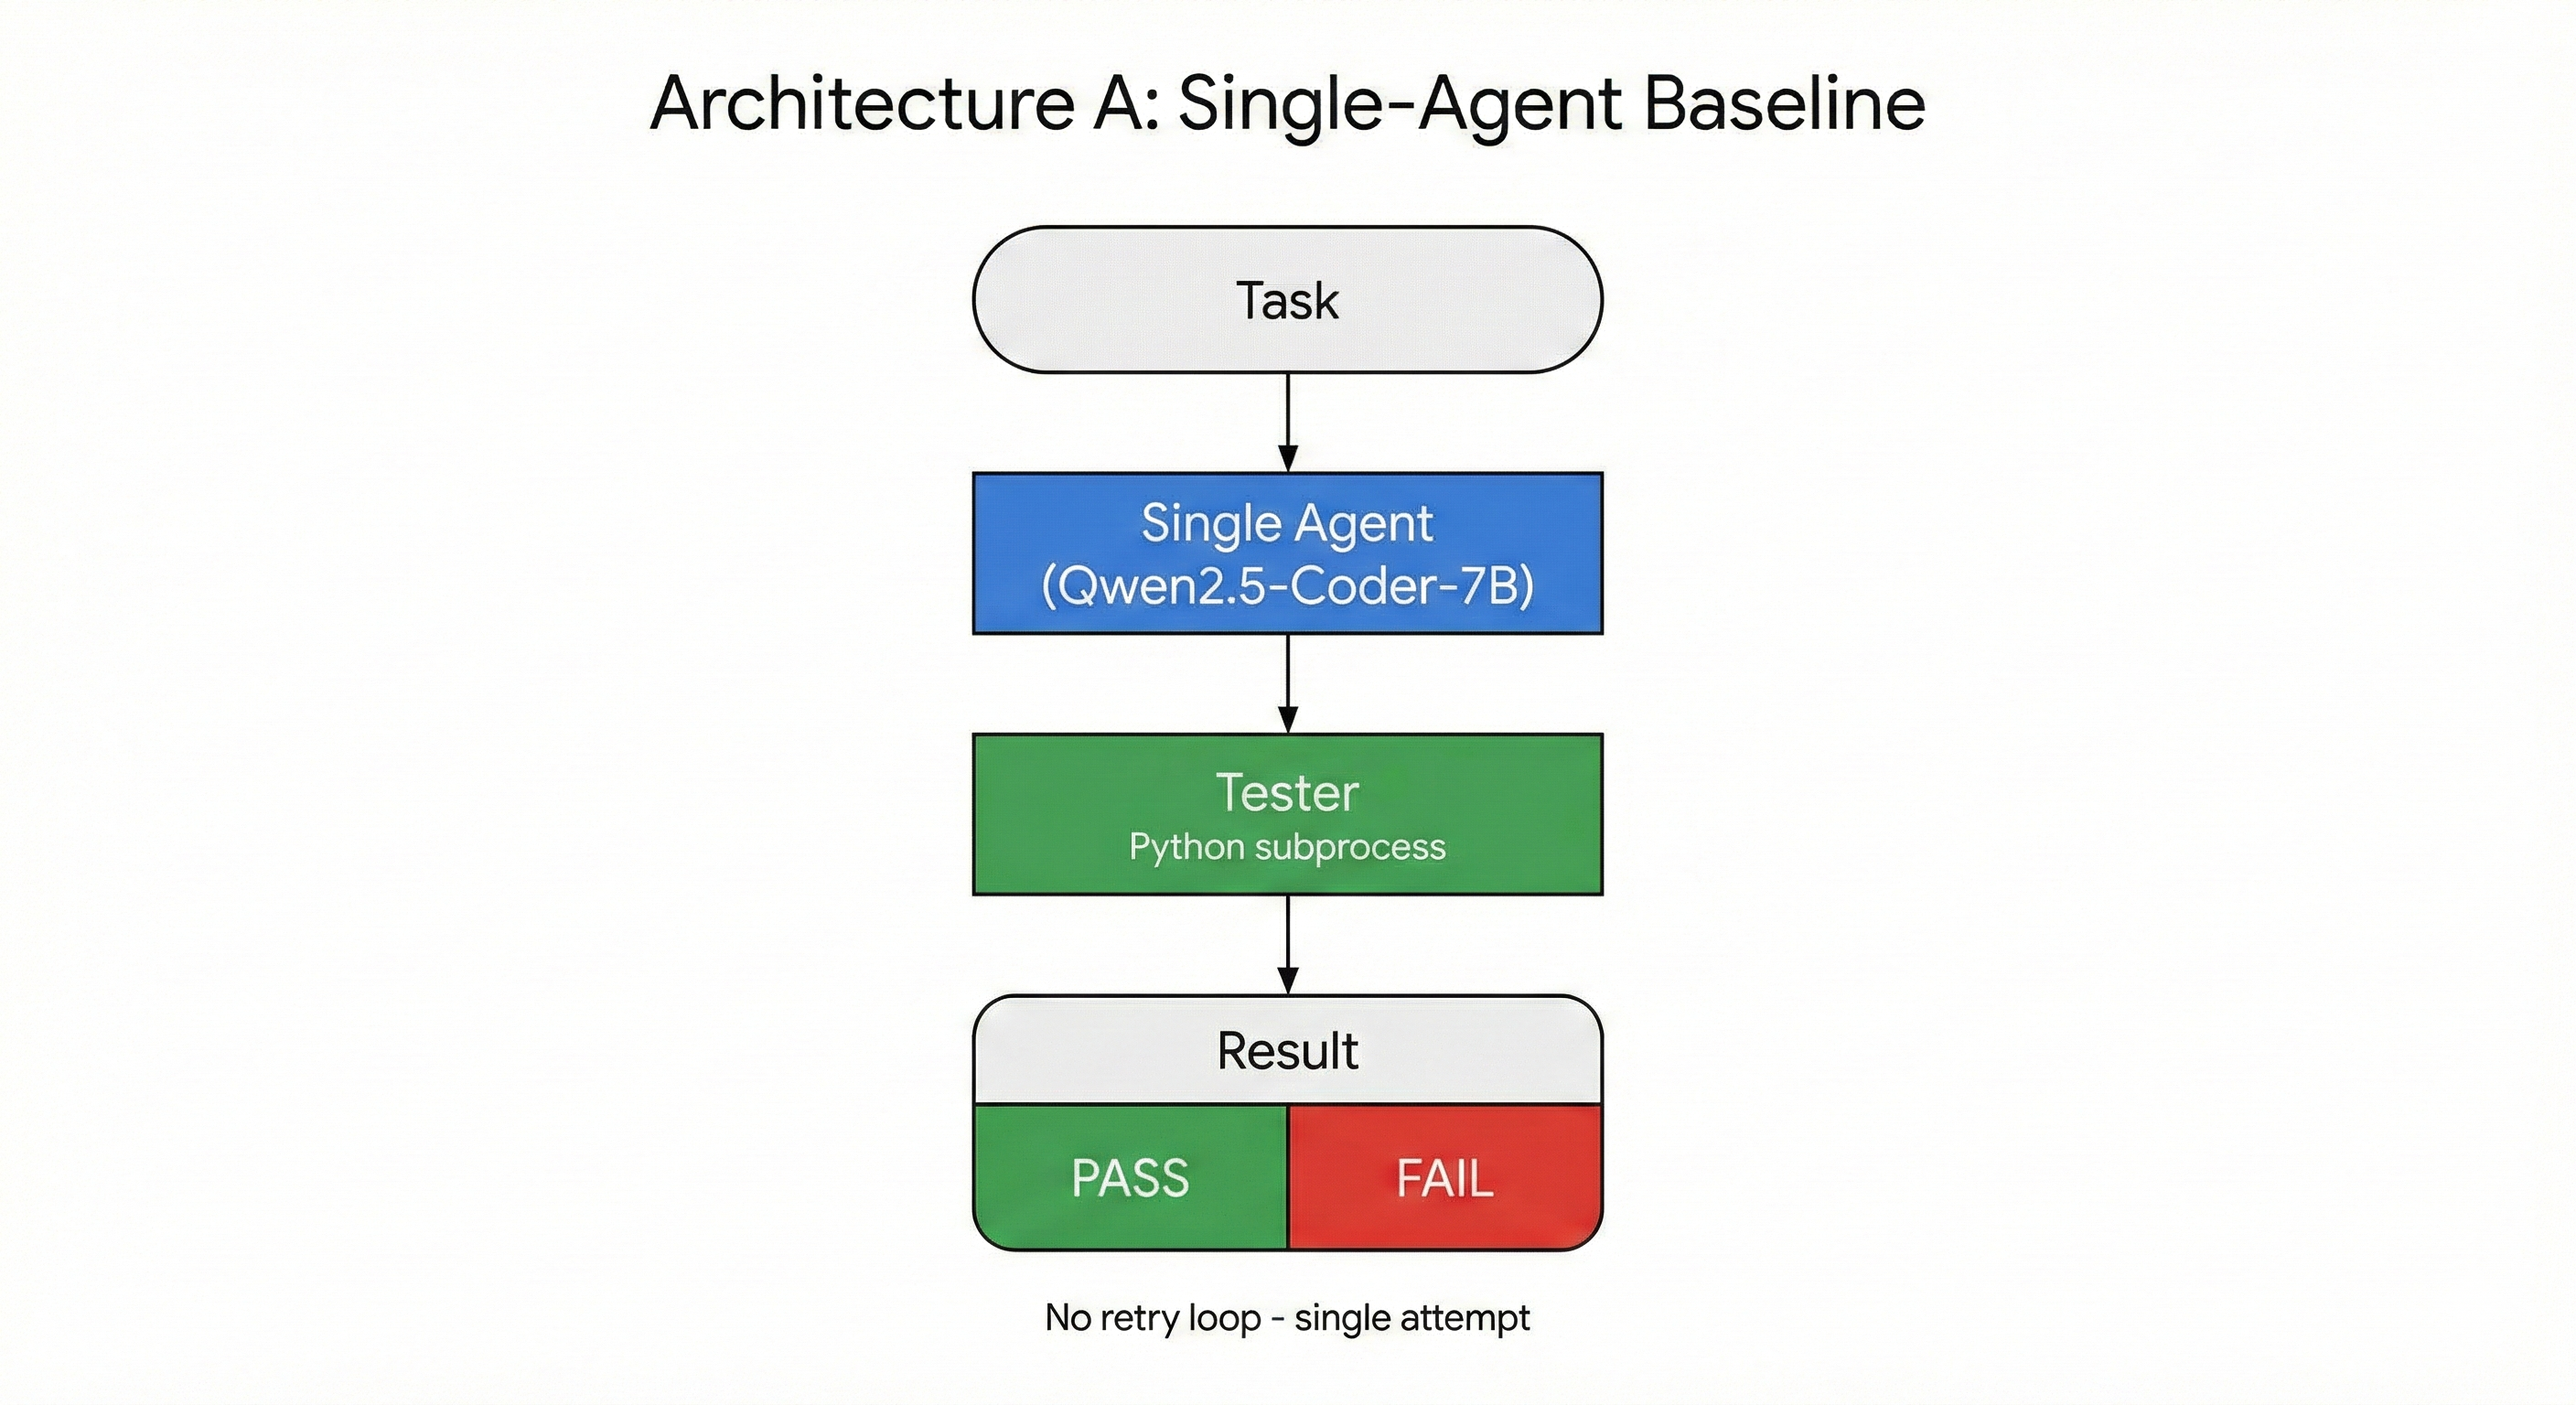
\includegraphics[width=\linewidth]{figures/SingleModel.png}
        \caption{Architecture A (Single Agent)}
        \label{fig:arch_a}
    \end{subfigure}
    
    \vspace{0.5em}
    
    \begin{subfigure}[b]{0.8\columnwidth}
        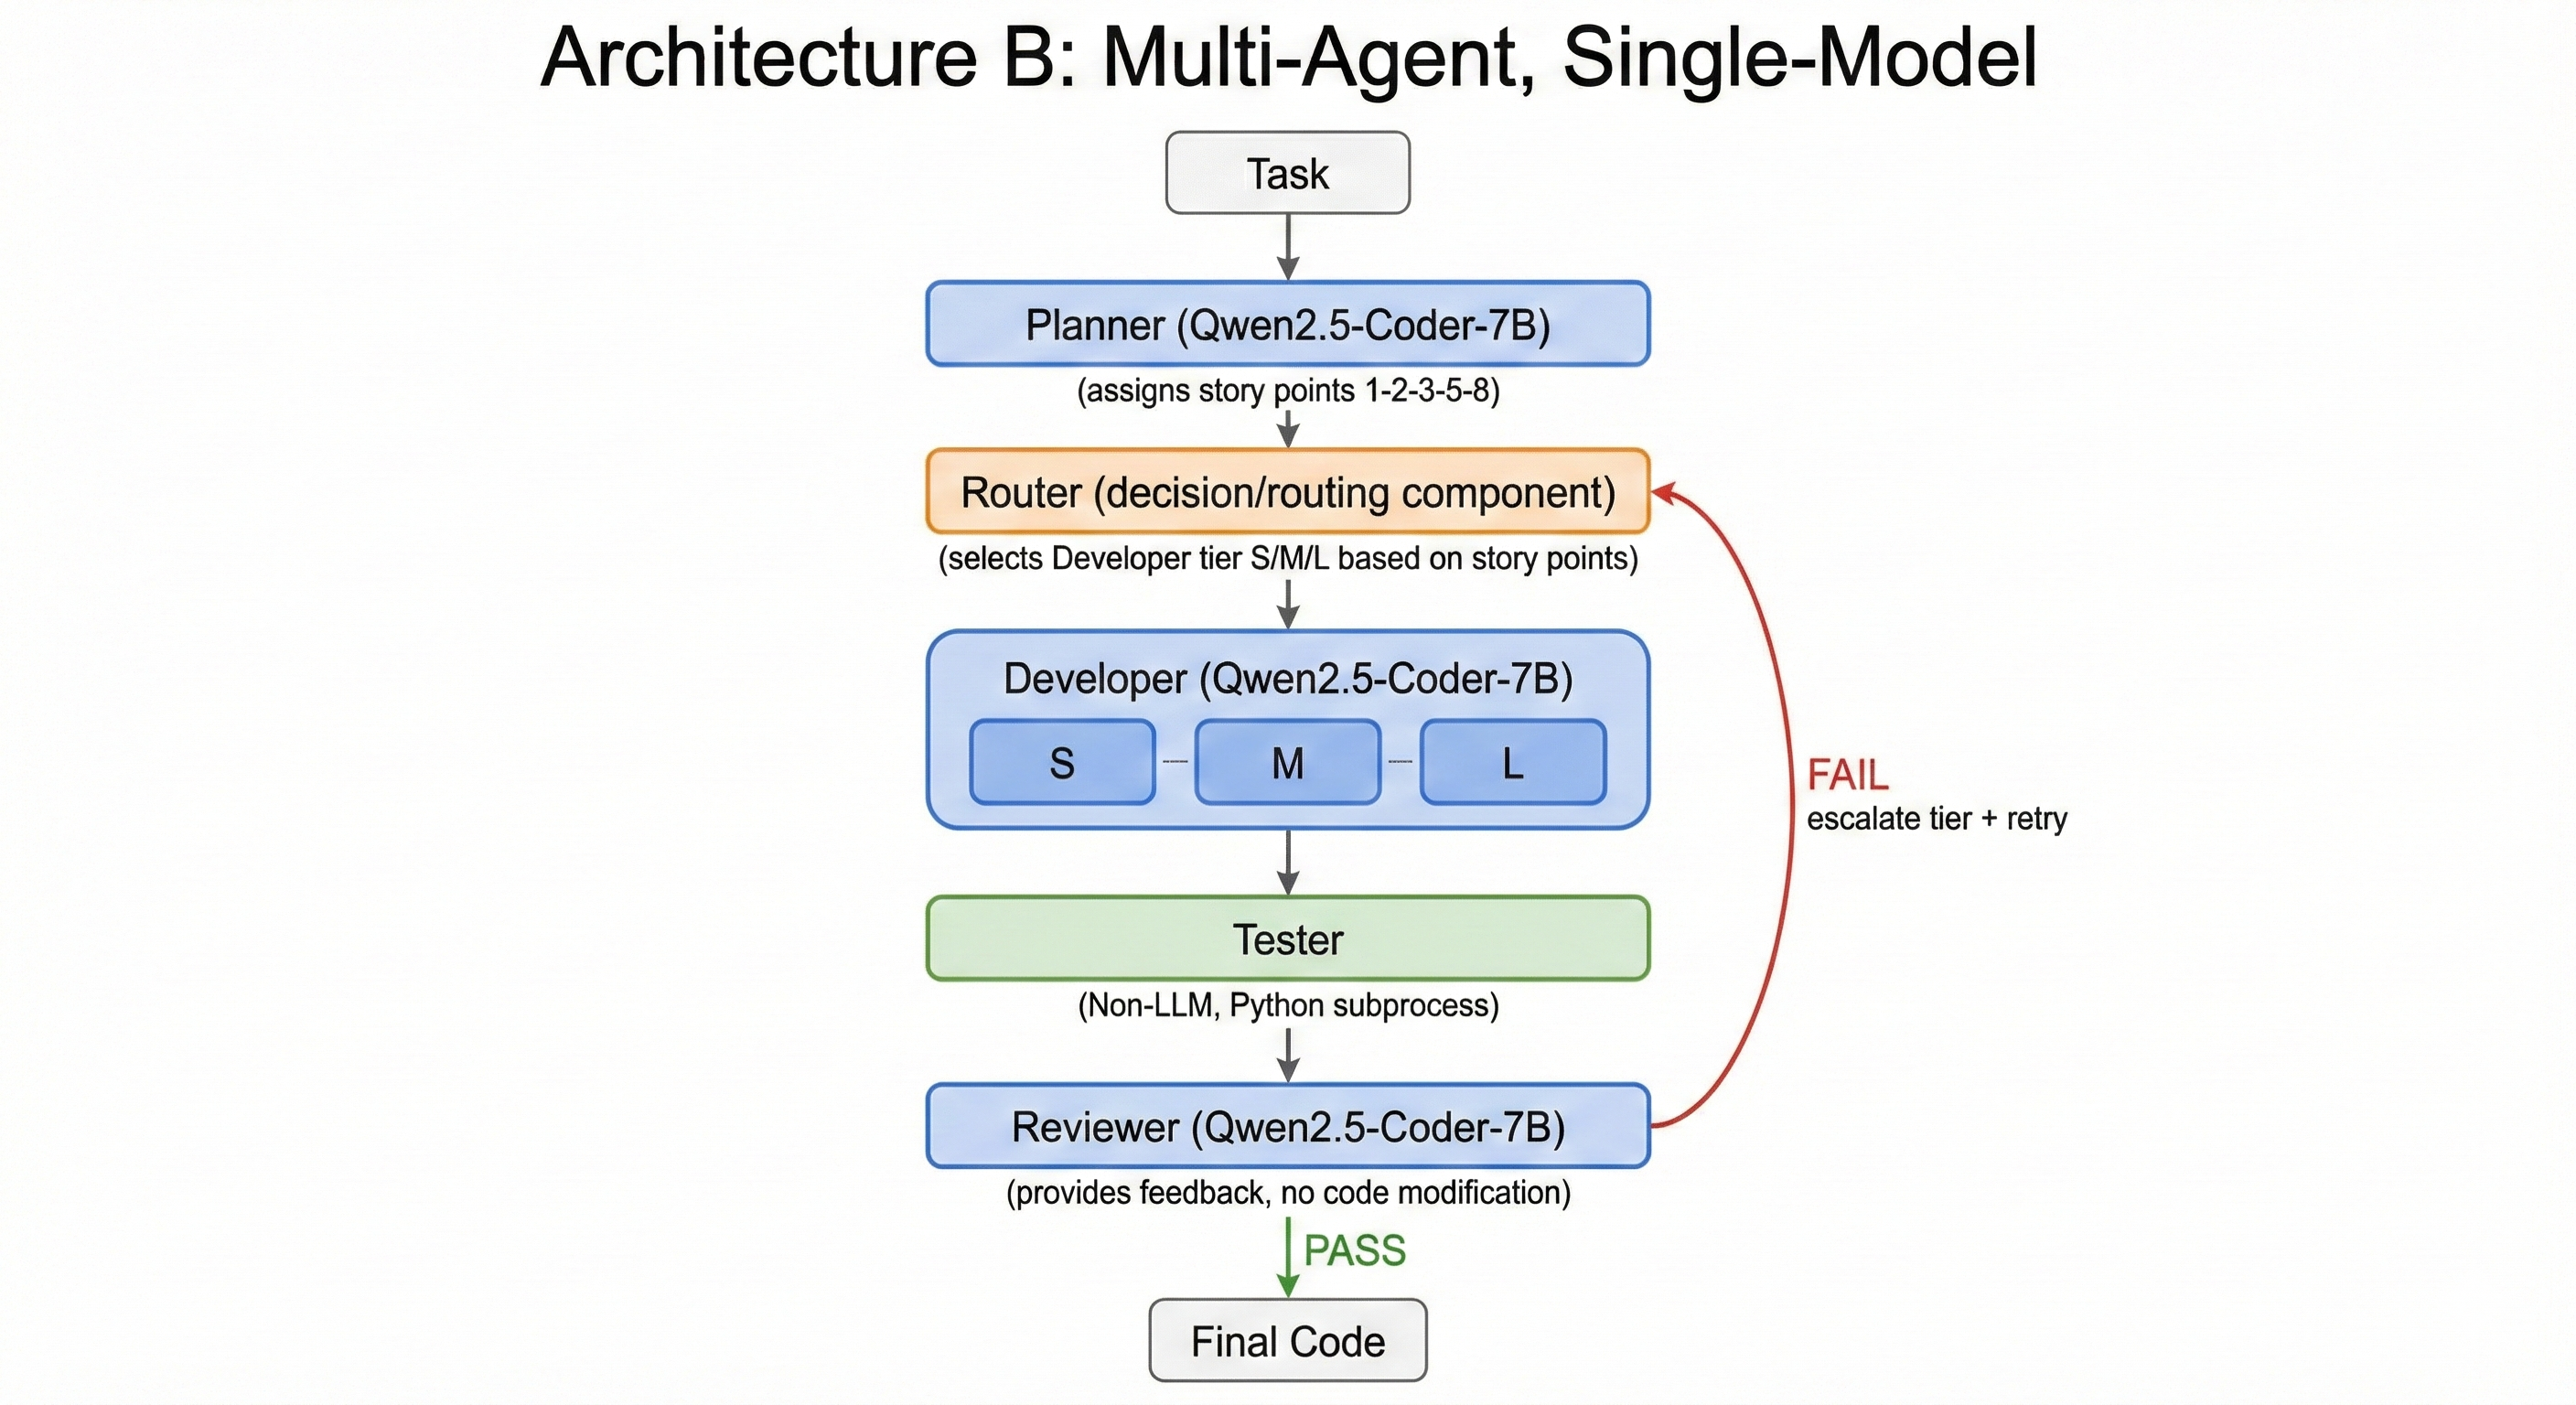
\includegraphics[width=\linewidth]{figures/MultiAgentSingleModel.png}
        \caption{Architecture B (Multi-Agent)}
        \label{fig:arch_b}
    \end{subfigure}
    \caption{Structural comparison of Single-Agent vs Multi-Agent architectures. Architecture B includes Planner, Router, Developer, Tester, and Reviewer nodes with a conditional retry loop.}
    \label{fig:rq1_architectures}
\end{figure}

The cost of this improvement is reflected in execution time: Architecture B averaged 10.95 seconds per task compared to 2.98 seconds for Architecture A, representing a 3.7$\times$ increase in latency. This overhead stems from the additional LLM calls (Planner, Reviewer) and potential retry iterations.

% -----------------------------------------------------------------------------
\subsection{RQ2: Effect of Specialized Models}
\label{subsec:rq2_results}

Next, we evaluate whether assigning specialized models to each role provides benefits over using a single generalist model. We compare \textbf{Architecture B} (Single-Model) with \textbf{Architecture C} (Multi-Model), where the latter uses Llama-3-8B for Planning and Reviewing, and a tiered set of Qwen models (1.5B, 7B, 32B) for development based on estimated task difficulty.

As shown in Table~\ref{tab:rq2_results}, Architecture C achieved a pass rate of \textbf{62.2\%}, which is surprisingly lower than the single-model Architecture B (72.6\%).

\begin{table}[ht]
    \centering
    \caption{Comparison of Single-Model (B) vs Multi-Model (C) Architectures.}
    \label{tab:rq2_results}
    \resizebox{\columnwidth}{!}{
    \begin{tabular}{lcccc}
        \toprule
        \textbf{Architecture} & \textbf{Pass Rate} & \textbf{95\% CI} & \textbf{Pass@1} & \textbf{Avg Time (s)} \\
        \midrule
        B (Single-Model) & \textbf{72.6\%} & [65.3, 78.8] & 50.6\% & 10.95 \\
        C (Multi-Model)  & 62.2\% & [54.6, 69.3] & 35.4\% & 19.28 \\
        \bottomrule
    \end{tabular}
    }
\end{table}

This counter-intuitive result can be attributed primarily to the performance of the smallest developer model (Tier S). In Architecture C, tasks estimated as "Easy" (Story Points 1--2) are routed to the Qwen-1.5B model. As detailed in the In-Depth Analysis (Section~\ref{subsec:indepth}), tasks initially routed to Tier S consistently failed, requiring escalation through the entire tier hierarchy. The 1.5B parameter model appears insufficient for reliable code generation in this framework, even for simple tasks.

Additionally, the coordination overhead between different model families (Llama for planning/review, Qwen for development) may have introduced subtle prompt-format incompatibilities or reasoning style mismatches that hurt overall coherence.

\begin{figure}[ht]
    \centering
    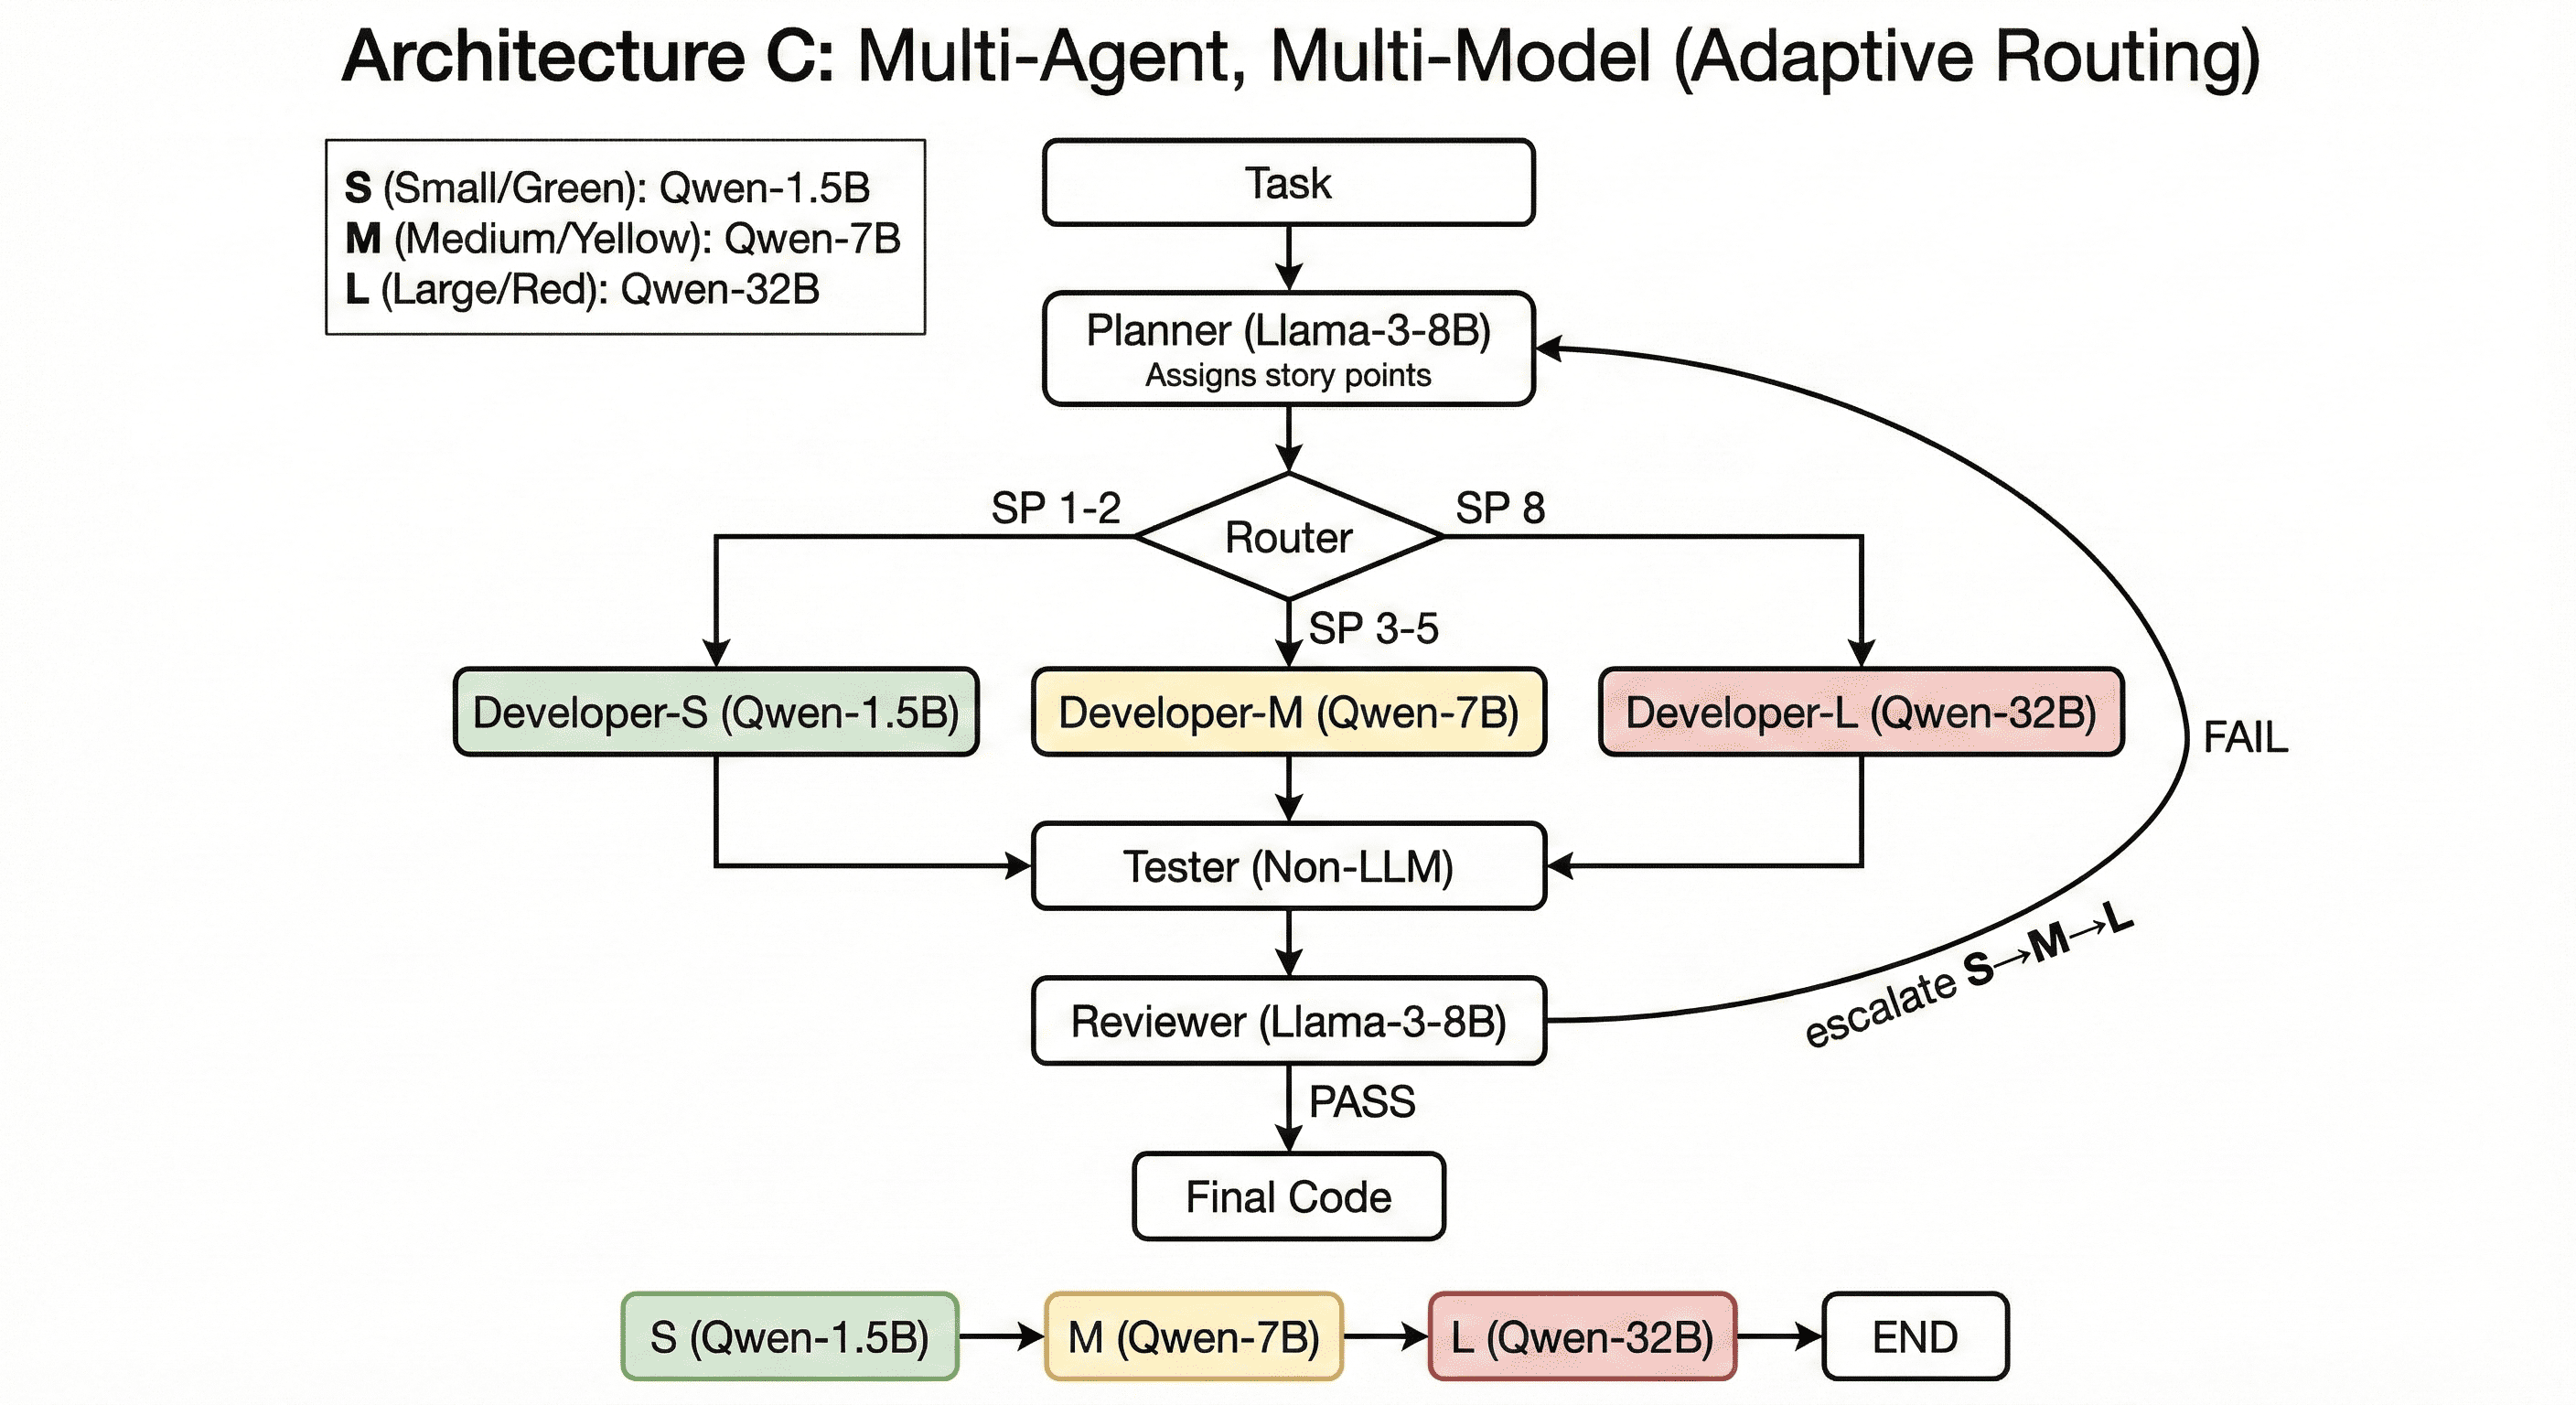
\includegraphics[width=0.65\columnwidth]{figures/MultiAgentMultiModel.png}
    \caption{Architecture C: Multi-Agent with specialized models per role and adaptive tier routing.}
    \label{fig:arch_c}
\end{figure}

% -----------------------------------------------------------------------------
\subsection{RQ3: Effect of Adaptive Routing}
\label{subsec:rq3_results}

To isolate the impact of adaptive routing from model specialization, we compare \textbf{Architecture C} (Adaptive S/M/L) with \textbf{Architecture C1} (Always-Large), as defined in Section~\ref{subsec:architectures}. In C1, the Router ignores story point estimates and always assigns tasks to the strongest available model (Qwen-32B).

Table~\ref{tab:rq3_results} presents a stark contrast. Architecture C1 achieved the highest pass rate in our study at \textbf{81.7\%}, significantly outperforming the adaptive version (62.2\%) by 19.5 percentage points.

\begin{table}[ht]
    \centering
    \caption{Comparison of Adaptive Routing (C) vs Always-Large (C1).}
    \label{tab:rq3_results}
    \resizebox{\columnwidth}{!}{
    \begin{tabular}{lcccc}
        \toprule
        \textbf{Architecture} & \textbf{Pass Rate} & \textbf{Avg Time (s)} & \textbf{Avg API Calls} & \textbf{Total Time (s)} \\
        \midrule
        C (Adaptive)  & 62.2\% & 19.28 & 4.85 & 3163 \\
        C1 (Always-L) & \textbf{81.7\%} & \textbf{14.66} & \textbf{3.00} & \textbf{2405} \\
        \bottomrule
    \end{tabular}
    }
\end{table}

Contrary to expectations, adaptive routing proved to be both less accurate \textit{and} more expensive than the Always-Large strategy. Architecture C consumed more time (19.28s vs 14.66s) and API calls (4.85 vs 3.00) on average because the adaptive approach frequently started with weaker models, failed, and then escalated through multiple retry loops. Architecture C1, by consistently using the most capable model, solved tasks on the first attempt 81.7\% of the time, avoiding costly retry overhead entirely.

\begin{figure}[ht]
    \centering
    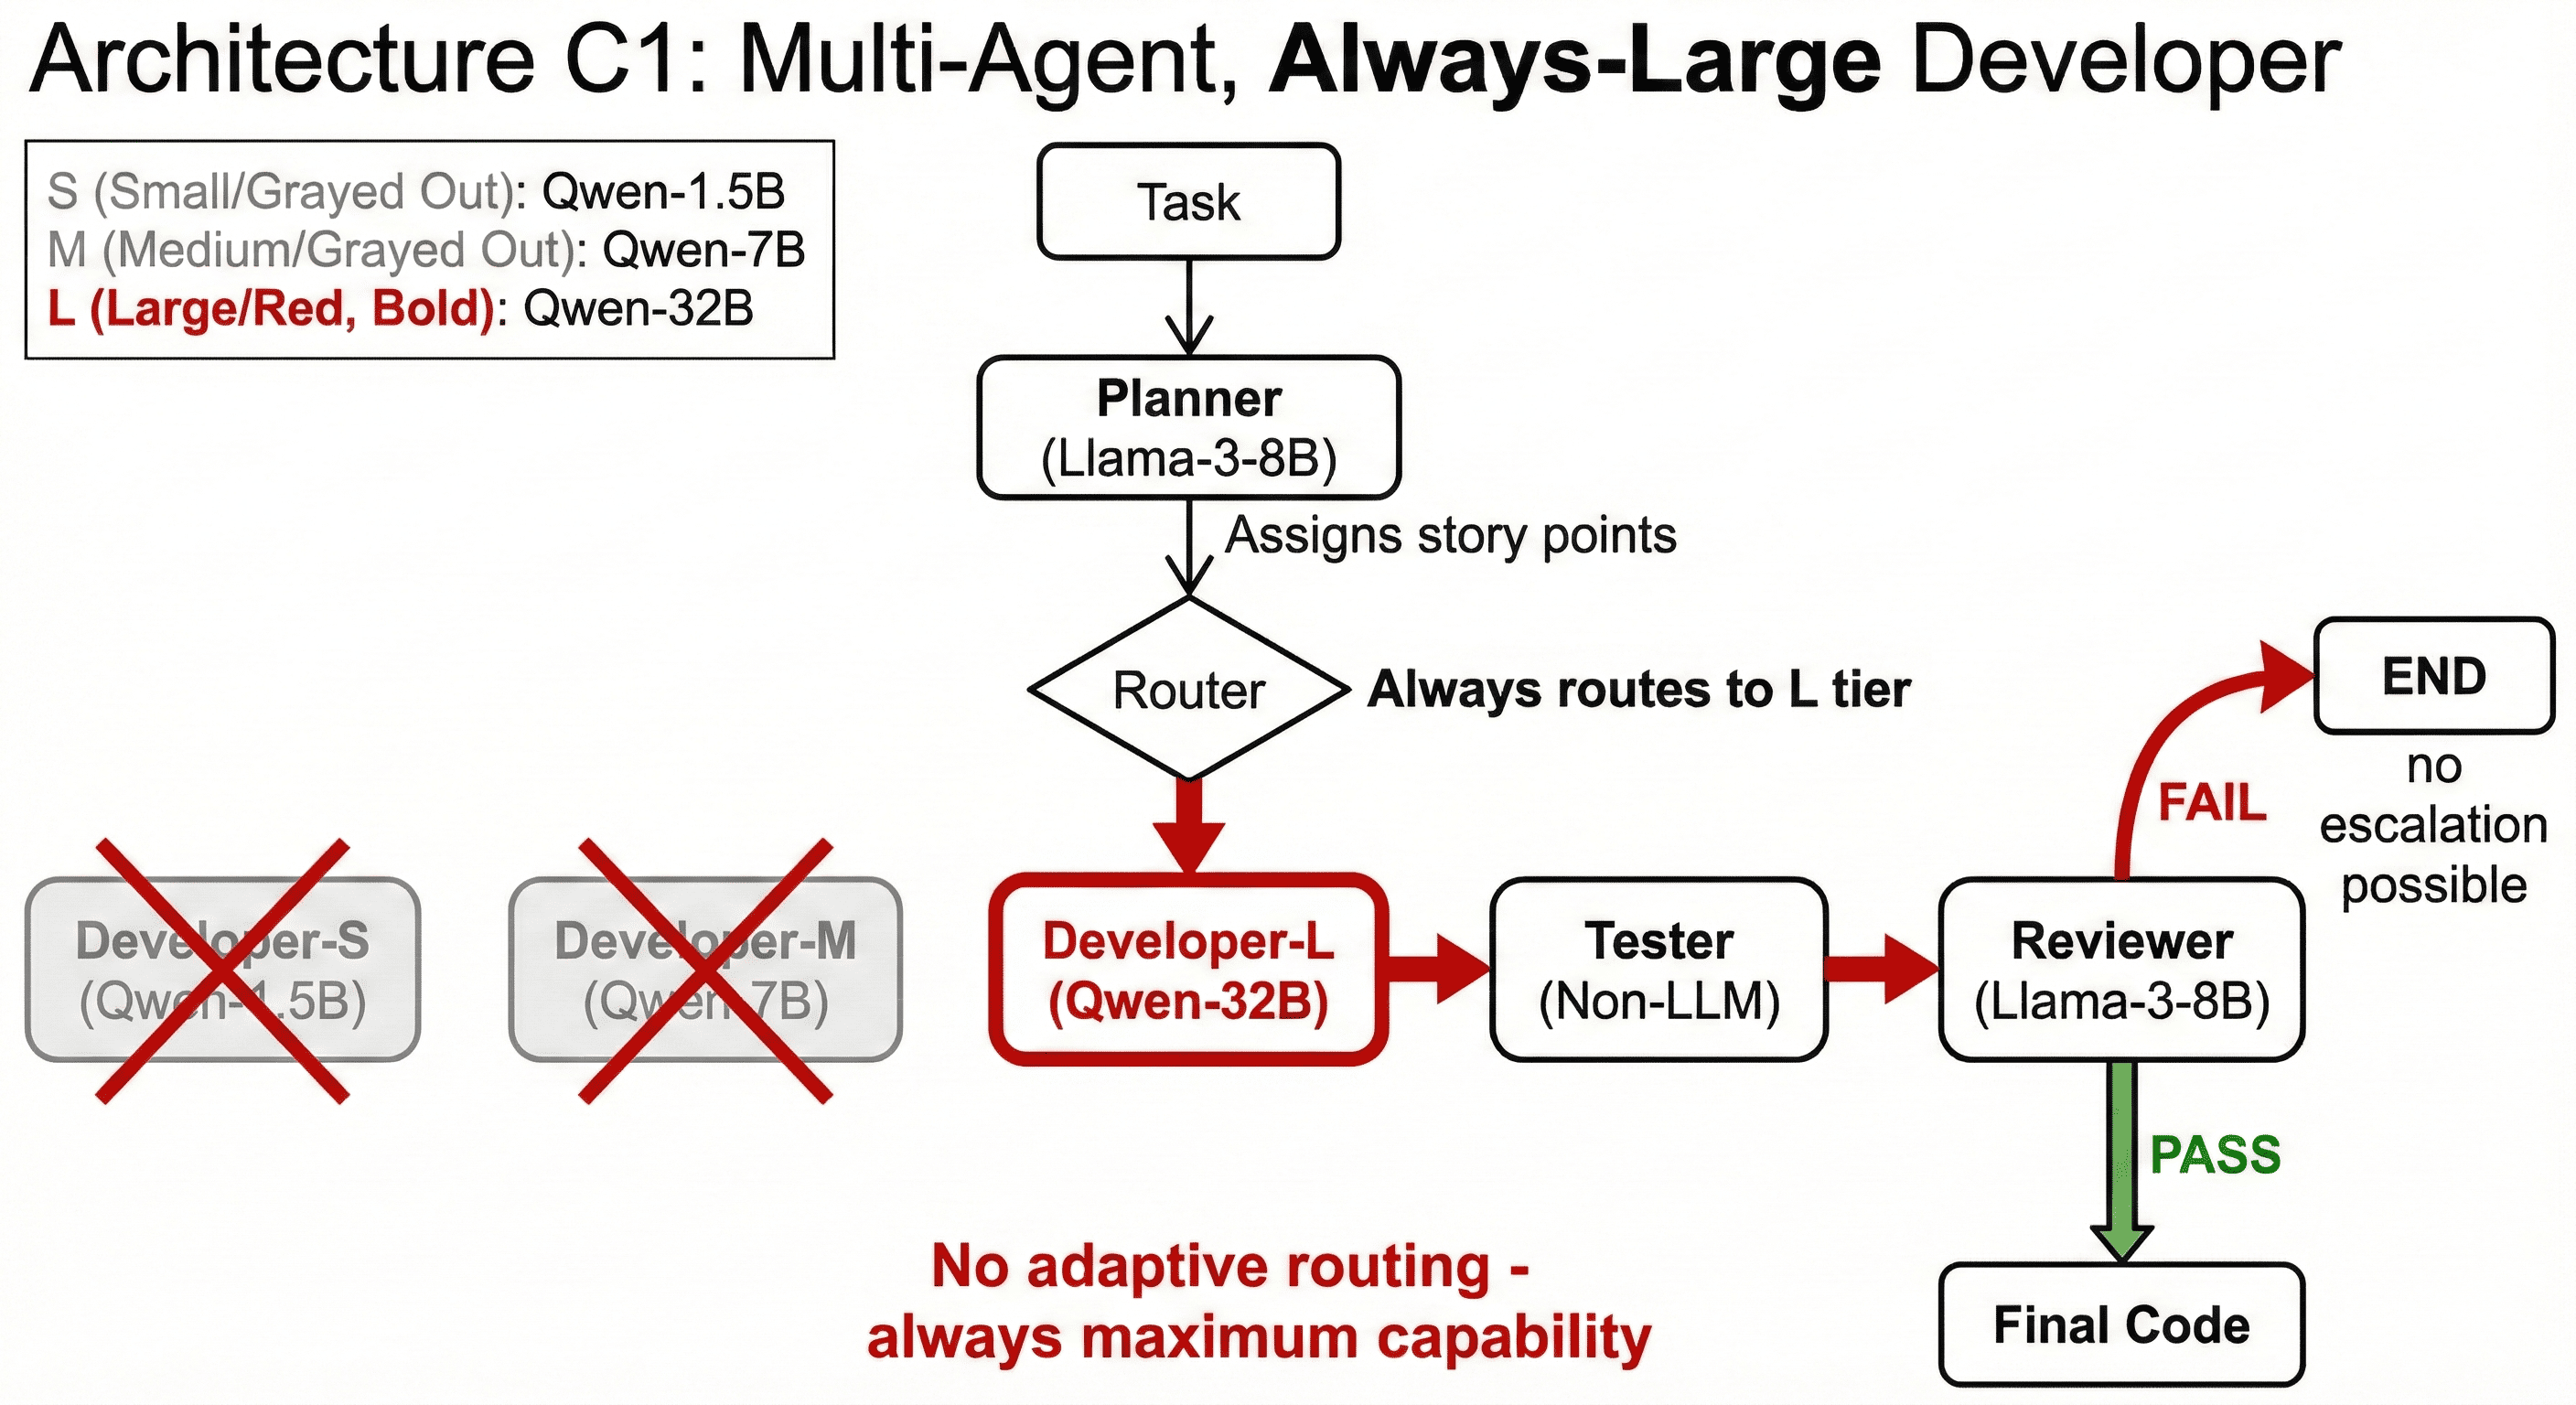
\includegraphics[width=0.65\columnwidth]{figures/MultiAgentAlwaysL.png}
    \caption{Architecture C1: Multi-Agent always routed to the largest (32B) developer model.}
    \label{fig:arch_c1}
\end{figure}

These results illustrate an interesting outcome for this specific configuration: attempting to save computational resources by using smaller models for easier tasks resulted in higher overall latency and dramatically lower success rates due to the frequency of required escalations and re-generations.

\paragraph{Ablation Study: Removing Tier S.}
To further investigate the role of the smallest model, we conducted an ablation study (Architecture C2, see Section~\ref{subsec:architectures}) where Tier S was removed entirely. Table~\ref{tab:ablation_c2} compares the results.

\begin{table}[ht]
    \centering
    \caption{Ablation Study: Removing Tier S (C2) vs Full Adaptive (C).}
    \label{tab:ablation_c2}
    \resizebox{\columnwidth}{!}{
    \begin{tabular}{lccc}
        \toprule
        \textbf{Architecture} & \textbf{Pass Rate} & \textbf{Avg Time (s)} & \textbf{Escalations} \\
        \midrule
        C (With Tier S)  & 62.2\% & 19.28 & 152 \\
        C2 (No Tier S)   & \textbf{72.0\%} & 13.32 & 74 \\
        \bottomrule
    \end{tabular}
    }
\end{table}

Architecture C2 achieved a pass rate of \textbf{72.0\%}, a substantial improvement of 9.8 percentage points over C. The removal of Tier S reduced total escalations from 152 to 74 and decreased average execution time from 19.28s to 13.32s. This confirms that the Qwen-1.5B model (Tier S) was the primary bottleneck in the adaptive configuration---its consistent failures triggered cascading escalations that consumed resources and polluted the context for subsequent attempts.

% -----------------------------------------------------------------------------
\subsection{RQ4: Effect of Prompt Repetition}
\label{subsec:rq4_results}

We evaluated the Prompt Repetition technique proposed by Leviathan et al.~\cite{leviathan2025prompt} across all base architectures. This technique duplicates the user prompt content to allow tokens in the second occurrence to attend to all tokens in the first occurrence, potentially improving comprehension of complex instructions.

Table~\ref{tab:rq4_results} summarizes the effect of prompt repetition on pass rates.

\begin{table}[ht]
    \centering
    \caption{Effect of Prompt Repetition on Pass Rates.}
    \label{tab:rq4_results}
    \resizebox{\columnwidth}{!}{
    \begin{tabular}{lccc}
        \toprule
        \textbf{Base Architecture} & \textbf{Standard} & \textbf{With -PR} & \textbf{Delta} \\
        \midrule
        A (Single-Agent) & 67.7\% & 68.3\% & +0.6\% \\
        B (Multi-Agent, Single-Model)  & 72.6\% & 66.5\% & --6.1\% \\
        C (Multi-Agent, Multi-Model)  & 62.2\% & 54.3\% & --7.9\% \\
        \bottomrule
    \end{tabular}
    }
\end{table}

Our findings diverge from those reported in the original paper. While the single-agent baseline (A) showed a negligible improvement (+0.6\%), the multi-agent architectures (B and C) experienced significant performance degradation (--6.1\% and --7.9\%, respectively).

A plausible explanation is that prompt repetition increases input context length substantially. In multi-agent pipelines, the conversation history already accumulates Planner outputs, previous code attempts, test error messages, and Reviewer feedback. Duplicating the user prompt in this already-rich context may introduce noise and make it harder for the model to attend to the most critical, recent instructions; particularly the specific feedback from the Reviewer explaining why the previous attempt failed.

This suggests that prompt repetition, while beneficial for simpler single-turn tasks, may be counterproductive in complex, multi-turn agentic workflows where context management is critical.

% -----------------------------------------------------------------------------
\subsection{In-Depth Analysis}
\label{subsec:indepth}

\paragraph{Escalation Patterns.}
Table~\ref{tab:escalation_analysis} presents the distribution of escalation counts and their corresponding pass rates across architectures.

\begin{table}[ht]
    \centering
    \caption{Escalation Analysis by Architecture.}
    \label{tab:escalation_analysis}
    \footnotesize
    \resizebox{\columnwidth}{!}{
    \begin{tabular}{lcccccc}
        \toprule
        \textbf{Arch} & \textbf{0-Esc} & \textbf{0-Esc Pass\%} & \textbf{1-Esc} & \textbf{1-Esc Pass\%} & \textbf{2-Esc} & \textbf{2-Esc Pass\%} \\
        \midrule
        B & 83 & 100\% & 53 & 62.3\% & 28 & 10.7\% \\
        C & 59 & 98.3\% & 58 & 31.0\% & 47 & 55.3\% \\
        C1 & 164 & 81.7\% & 0 & --- & 0 & --- \\
        \bottomrule
    \end{tabular}
    }
\end{table}

In Architecture B, tasks that passed without escalation achieved 100\% success, but success dropped sharply with each escalation level (62.3\% at 1-Esc, 10.7\% at 2-Esc). Architecture C exhibited a similar pattern but with an unusual recovery at 2-Esc (55.3\%), suggesting that the strongest Tier L model (32B) could rescue some tasks that Tier M could not.

\paragraph{Developer Tier Distribution.}
Table~\ref{tab:tier_distribution} shows the final tier assignment for each architecture.

\begin{table}[ht]
    \centering
    \caption{Developer Tier Distribution (Final Assignment).}
    \label{tab:tier_distribution}
    \footnotesize
    \resizebox{\columnwidth}{!}{
    \begin{tabular}{lccc|ccc}
        \toprule
        & \multicolumn{3}{c|}{\textbf{Count (\%)}} & \multicolumn{3}{c}{\textbf{Pass Rate at Tier}} \\
        \textbf{Architecture} & \textbf{S} & \textbf{M} & \textbf{L} & \textbf{S} & \textbf{M} & \textbf{L} \\
        \midrule
        B & 57 (35\%) & 53 (32\%) & 54 (33\%) & 100\% & 100\% & 16.7\% \\
        C & 0 (0\%) & 57 (35\%) & 107 (65\%) & --- & 100\% & 42.1\% \\
        C1 & 0 (0\%) & 0 (0\%) & 164 (100\%) & --- & --- & 81.7\% \\
        \bottomrule
    \end{tabular}
    }
\end{table}

In Architecture C, no tasks completed at Tier S, all initially routed S-tier tasks escalated. This confirms that the Qwen-1.5B model is inadequate for this code generation framework. Notably, the Tier L pass rate in Architecture C (42.1\%) is much lower than in C1 (81.7\%), indicating that accumulated errors from prior failed attempts may have polluted the context for subsequent generations.

\paragraph{Story Point Accuracy.}
The Planner's story point estimates showed limited predictive power. In Architecture C1, tasks assigned SP=1-2 (trivial) achieved 86--100\% pass rates, while SP=8 (hard) tasks achieved only 50\%. This suggests the Planner's difficulty estimates have some validity, but the benefit of adaptive routing was negated by the weakness of smaller-tier models.

% -----------------------------------------------------------------------------
\subsection{Static Code Quality Analysis}
\label{subsec:code_quality}

We analyzed the quality of generated code using Cyclomatic Complexity (CC) and Maintainability Index (MI), computed via the Radon library.

\begin{table}[ht]
    \centering
    \caption{Static Code Quality Metrics by Architecture.}
    \label{tab:code_quality}
    \resizebox{\columnwidth}{!}{
    \begin{tabular}{lcc|cc}
        \toprule
        & \multicolumn{2}{c|}{\textbf{Overall}} & \multicolumn{2}{c}{\textbf{Passed vs Failed}} \\
        \textbf{Architecture} & \textbf{Avg CC} & \textbf{Avg MI} & \textbf{Passed CC} & \textbf{Failed CC} \\
        \midrule
        A (Single) & 3.59 & 75.0 & 3.67 & 3.21 \\
        B (Multi, Single-Model)  & 3.87 & 84.5 & 3.76 & 4.66 \\
        C (Multi, Multi-Model)  & 3.84 & 85.4 & 4.02 & 3.08 \\
        C1 (Always-L) & 4.58 & 81.1 & 4.55 & 4.85 \\
        \bottomrule
    \end{tabular}
    }
\end{table}

Several observations emerge from Table~\ref{tab:code_quality}:

\begin{itemize}
    \item \textbf{Multi-agent architectures produce more maintainable code.} Architectures B and C achieved MI scores above 84, compared to 75 for the single-agent baseline. This suggests the review process encourages cleaner code structures.
    \item \textbf{The strongest model produces more complex code.} Architecture C1's average CC (4.58) was highest, potentially reflecting more sophisticated algorithmic solutions.
    \item \textbf{Failed tasks in Architecture B show higher complexity.} The CC for failed tasks (4.66) exceeds that of passed tasks (3.76), indicating the model struggled with inherently complex problems.
\end{itemize}

All architectures maintained CC values in the "low risk" range (1--5), and MI values above 75 indicate "high maintainability" according to standard thresholds.
